% !TeX root = main.tex
\documentclass[11pt,a4paper]{article}
% \documentclass[a4paper,14pt, draft]{article}

%%% отключение нумерации сраниц
\pagestyle{empty}
%%% значок в itemize
% \renewcommand{\labelitemi}{$\cdot$}

%%% Работа с русским языком
\usepackage{cmap}					% поиск в PDF
\usepackage{mathtext} 				% русские буквы в формулах
\usepackage[T1, T2A]{fontenc}			% кодировка %Т1 посоветовал чат гпт
\usepackage[utf8]{inputenc}			% кодировка исходного текста
\usepackage[english,russian]{babel}	% локализация и переносы
\usepackage{indentfirst}            % красная строка в первом абзаце
\frenchspacing                      % равные пробелы между словами и предложениями

%%% Дополнительная работа с математикой
\usepackage{amsmath,amsfonts,amssymb,amsthm,mathtools} % пакеты AMS
\usepackage{icomma}                                    % "Умная" запятая

%%% Свои символы и команды
\usepackage{centernot} % центрированное зачеркивание символа
\usepackage{stmaryrd}  % некоторые спецсимволы
\usepackage{dsfont}
\usepackage{amsthm}


\renewcommand{\epsilon}{\ensuremath{\varepsilon}}
\renewcommand{\phi}{\ensuremath{\varphi}}
\renewcommand{\kappa}{\ensuremath{\varkappa}}
\renewcommand{\le}{\ensuremath{\leqslant}}
\renewcommand{\leq}{\ensuremath{\leqslant}}
\renewcommand{\ge}{\ensuremath{\geqslant}}
\renewcommand{\geq}{\ensuremath{\geqslant}}
\renewcommand{\emptyset}{\ensuremath{\varnothing}}

\DeclareMathOperator{\sgn}{sgn}
\DeclareMathOperator{\ke}{Ker}
\DeclareMathOperator{\im}{Im}
\DeclareMathOperator{\re}{Re}

\newcommand{\N}{\mathbb{N}}
\newcommand{\Z}{\mathbb{Z}}
\newcommand{\Q}{\mathbb{Q}}
\newcommand{\R}{\mathbb{R}}
\newcommand{\Cm}{\mathbb{C}}
\newcommand{\F}{\mathbb{F}}
\newcommand{\id}{\mathrm{id}}
\newcommand{\imp}[2]{
	(#1\,\,$\ra$\,\,#2)\,\,
}
\newcommand{\Root}[2]{
	\left\{\!\sqrt[#1]{#2}\right\}
}
\newcommand{\RR}{\R}
\newcommand{\NN}{\N}
\renewcommand{\subseteq}{\subset}
\newcommand{\sub}{\subset}
\newcommand{\sconstr}{\;\vert\;}
\newcommand{\thus}{\implies}

\newcommand{\defeq}{\vcentcolon= }
\newcommand{\defev}{\stackrel{\Delta}{\Longleftrightarrow}}
\newcommand{\deriv}[3][1]{%
	\ifthenelse{#1>1}{%
		\frac{\dlta^{#1} {#2}}{\dlta {#3}^{#1}}
	}{%
		\frac{\dlta {#2}}{\dlta {#3}}
	}%
}

\renewcommand\labelitemi{$\triangleright$}

\let\bs\backslash
\let\lra\Leftrightarrow
\let\ra\Rightarrow
\let\la\Leftarrow
\let\emb\hookrightarrow

%%% Перенос знаков в формулах (по Львовскому)
\newcommand{\hm}[1]{#1\nobreak\discretionary{}{\hbox{$\mathsurround=0pt #1$}}{}}

%%% Работа с картинками
\usepackage{graphicx}    % Для вставки рисунков
\setlength\fboxsep{3pt}  % Отступ рамки \fbox{} от рисунка
\setlength\fboxrule{1pt} % Толщина линий рамки \fbox{}
\usepackage{wrapfig}     % Обтекание рисунков текстом

% \usepackage[inkscapeformat=png]{svg} %% svg

%%% Работа с таблицами
\usepackage{array,tabularx,tabulary,booktabs} % Дополнительная работа с таблицами
\usepackage{longtable}                        % Длинные таблицы
\usepackage{multirow}                         % Слияние строк в таблице

%%% Теоремы
\theoremstyle{plain}
\newtheorem*{theorem}{Теорема}
\newtheorem*{lemma}{Лемма}
\newtheorem*{proposition}{Утверждение}
\newtheorem*{exercise}{Упражнение}
\newtheorem*{problem}{Задача}

\theoremstyle{definition}
\newtheorem*{definition}{Определение}
\newtheorem*{corollary}{Следствие}
\newtheorem*{note}{Замечание}
\newtheorem*{reminder}{Напоминание}
\newtheorem*{example}{Пример}

\theoremstyle{remark}
\newtheorem*{solution}{Решение}

%%% Оформление страницы
\usepackage{extsizes}     % Возможность сделать 14-й шрифт
\usepackage{geometry}     % Простой способ задавать поля
\usepackage{setspace}     % Интерлиньяж
\usepackage{enumitem}     % Настройка окружений itemize и enumerate
\setlist{leftmargin=10pt} % Отступы в itemize и enumerate

\geometry{top=15mm}    % Поля сверху страницы
\geometry{bottom=5mm} % Поля снизу страницы
\geometry{left=10mm}   % Поля слева страницы
\geometry{right=10mm}  % Поля справа страницы

\setlength\parindent{15pt}        % Устанавливает длину красной строки 15pt
\linespread{1}                  % Коэффициент межстрочного интервала
%\setlength{\parskip}{0.5em}      % Вертикальный интервал между абзацами
\setcounter{secnumdepth}{0}      % Отключение нумерации разделов
%\setcounter{section}{-1}         % Нумерация секций с нуля
\usepackage{multicol}			  % Для текста в нескольких колонках
\usepackage{soulutf8}             % Модификаторы начертания
\mathtoolsset{showonlyrefs=true} % показывать номера формул только у тех, у которых есть ссылки по eqref
%%% Содержаниие
% \usepackage{tocloft}
% \tocloftpagestyle{main}
%\setlength{\cftsecnumwidth}{2.3em}
%\renewcommand{\cftsecdotsep}{1}
%\renewcommand{\cftsecpresnum}{\hfill}
%\renewcommand{\cftsecaftersnum}{\quad}

%%% Нумерация уравнений
\makeatletter
\def\eqref{\@ifstar\@eqref\@@eqref}
\def\@eqref#1{\textup{\tagform@{\ref*{#1}}}}
\def\@@eqref#1{\textup{\tagform@{\ref{#1}}}}
\makeatother                      % \eqref* без гиперссылки
\numberwithin{equation}{section}  % Нумерация вида (номер_секции).(номер_уравнения)
\mathtoolsset{showonlyrefs= true} % Номера только у формул с \eqref{} в тексте.

%%% Гиперссылки
\usepackage{hyperref}
\usepackage[usenames,dvipsnames,svgnames,table,rgb]{xcolor}
\hypersetup{
	unicode=true,            % русские буквы в раздела PDF
	colorlinks=true,       	 % Цветные ссылки вместо ссылок в рамках
	linkcolor=black!15!blue, % Внутренние ссылки
	citecolor=green,         % Ссылки на библиографию
	filecolor=magenta,       % Ссылки на файлы
	urlcolor=NavyBlue,       % Ссылки на URL
}

%%% Графика
\usepackage{tikz}        % Графический пакет tikz
\usepackage{tikz-cd}     % Коммутативные диаграммы
\usepackage{tkz-euclide} % Геометрия
\usepackage{stackengine} % Многострочные тексты в картинках
\usetikzlibrary{angles, babel, quotes}
%%% значок в itemize
\renewcommand{\labelitemi}{$\multimap  $}
\title{\texttt{Определение энергии активации
по температурной зависимости вязкости
жидкости \\ 2.2.6}}
\author{}
\date{}

\begin{document}
  \maketitle

\textbf{Цель работы:}
\begin{itemize}
  \item  Измерение скорости падения шариков при разной
  температуре жидкости
  \item Вычисление вязкости жидкости по закону
  Стокса и расчёт энергии активации
\end{itemize}

\textbf{В работе используются:}  стеклянный цилиндр с исследуемой
 жидкостью (глицерин); термостат; секундомер; горизонтальный компаратор; 
 микроскоп; мелкие шарики (диаметром около 1 мм)

\section*{\texttt{Теория}}
В жидкостях, как и в кристаллах, каждая
молекула находится в потенциальной яме электрического поля, 
создаваемого окружающими молекулами. Молекулы колеблются со средней
частотой, близкой к частоте колебаний атомов в кристаллических телах
($\backsim 10^{12}$ Гц), с амплитудой, определяемой размерами объёма, 
предоставленного ей соседними молекулами. Глубина потенциальной ямы в
жидкостях больше средней кинетической энергии колеблющейся 
молекулы, поэтому молекулы колеблются вокруг более или 
менее стабильных положений равновесия. Однако у жидкостей различие 
между этими двумя энергиями невелико, так что молекулы нередко выскакивают из
"своей" потенциальной ямы и занимают место в другой.\\
Для перехода в новое состояние молекула должна получить
некоторое количество энергии W, называемую \textit{энергией мотивации}.\\
Температурная зависимость вязкости жидкости 
выражается формулой: \[\eta \backsim e^{W/kT}\]
Экспериментальные исследования показывают, что формула
неплохо работает в небольших температурных интервалах.\\
Формула Стокса для ламинарного обтекания шарика безграничной жидкостью:
\[F = 6\pi\eta rv \]
\fbox{Характер обтекания определяется числом 
Рейнольдса $Re = vr\rho_\text{ж} /\eta$ }(для ламинарного течения Re < 0.5)\\
Время релаксации скорости:
\[\tau = \frac{2}{9} \frac{r^2\rho}{\eta}\]
Тогда $\eta$:

\begin{center}
  \fbox{$\eta = \frac{2}{9}gr^2\frac{\rho - \rho_\text{ж}}{v_\text{уст}}$}
\end{center}

\newpage

\section*{Экспериментальная установка}
\subsection*{\texttt{Важные константы:}}
  \indent Диаметр сосуда:\\
  \indent Длина сосуда:\\
  \indent s = $(10.0 \pm 0.1) \text{см}$

\begin{figure}[h!]
  \includegraphics*[width=\textwidth]{ust.png}
  \caption{Установка для определения коэффициента
  вязкости жидкости}
  \label{fig:ust}
\end{figure}
% \noindent Схема экспериментальной установки представлена на рис~\ref{fig:ust}.

Измеряем пройденное расстояние линейкой, а время -- секундомером,
находим $v_\text{уст}$. Радиус шарика измеряем горизонтальным
компаратором/микроскопом (для каждого шарика измеряем насколько диаметров и берём среднее).
Плотность шариков и жидкости -- табличные значения.\\
Опыты проводятся при нескольких температурах в интервале от
комнатной до $320-330$ К.\\
Для каждой температуры проводим измерения с разными диаметрами шариков.\\
Построим график в координатах $ln(\eta) \bigl(T^{-1}\bigr)$.\\
Если во всем диапазоне встречающихся в работе 
скоростей и времён релаксации вычисленные по нашей формуле
значения $\eta$ оказываются одинаковыми, то формула Стокса правильно
передаёт зависимость сил от радиуса шарика.
Если всё-таки наблюдается кореляция $\eta$ и $r$, то нужно использовать формулу:
\begin{center}{
  \fbox{
  $\eta = \frac{2}{9}gr^2\frac{\rho - \rho_\text{ж}}{v_\text{уст}} \cdot \frac{1}{1 + 2.4(r/R)}$
}}\end{center}
где R --  радиус сосуда.
  
\section*{Ход работы}
\begin{enumerate}
  \setcounter{enumi}{-1}
  \item Отберём 24 шарика. Для каждого шарика измерим микроскопом
  диаметр в двух положениях и усредним.
  \item Измерим зависимость скорости падения шарика от температуры жидкости.
  Скорость измеряем по формуле $v_\text{уст} = s / t_\text{падения}$
  Для каждой температуры будем проводить измерения по 4-5 раз, фиксируя при этом изменение температуры.
  \item Для каждого из опытов вычислим число Рейнольдса, оценим время и путь релаксации,
  занесём всё в табличку.
  \item График зависимости $ln \eta  (T^{-1})$
  \begin{center}
    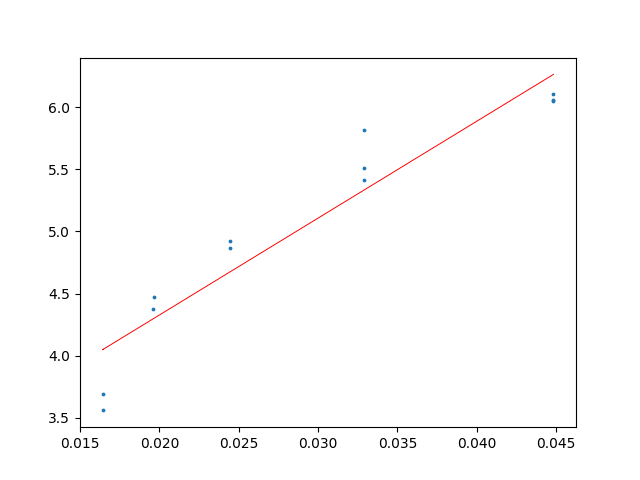
\includegraphics[width=0.9\textwidth]{graph steel.png}
    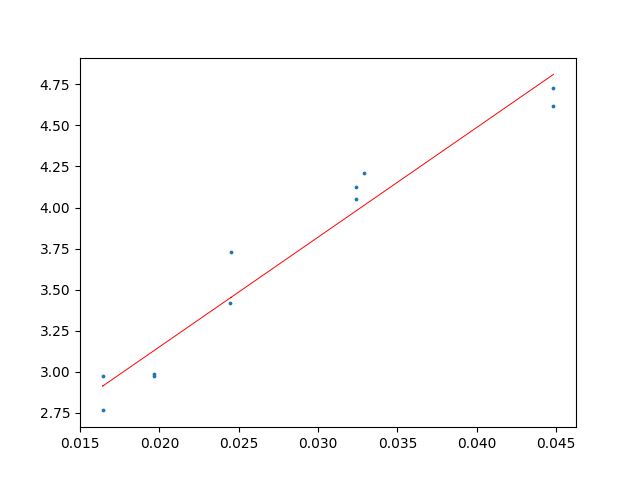
\includegraphics[width=0.9\textwidth]{graph glass.png}
  \end{center}
  Из МНК, среднеквадратичная ошибка для стекла меньше, чем для стали (0.0011 vs 0.0013), поэтому будем использовать
  значение энергии активации, полученной для стали
  \item Энергия активации:
  \[W = 6.67 * 10 ^ {-20}\frac{\text{Дж}}{\text{Моль}}\]
  \[\sigma_W =  6.14 * 10 ^ {-21}\]

\end{enumerate}
\section*{Вывод}

\end{document}
